\chapter{Progetto di Archivi Digitali}
\label{ch:archivi}

Questo capitolo contiene la documentazione del progetto realizzato utilizzando le tecnologie descritte nei capitoli precedenti. Si tratta di un’applicazione decentralizzata costruita attraverso la blockchain pubblica Ethereum e il protocollo IPFS. Lo scopo principale di questo progetto è la descrizione della metodologia di sviluppo in un ecosistema distribuito. Se per molti programmatori imparare un nuovo linguaggio di programmazione o framework può essere una situazione frequente, lo sviluppo in un paradigma differente richiede una descrizione più approfondita della metodologia e delle pratiche migliori da adottare durante la fase di preparazione e di sviluppo.

\section{Definizione di obiettivi e requisiti dell’applicazione}

L’obiettivo dell'applicazione consiste nello sviluppo di un registro contenete opere d’arte definibili come minori che, potranno essere memorizzate in maniera trasparente, permanente e immutabile in una blockchain pubblica.

In dettaglio l’applicazione deve soddisfare i seguenti requisiti e funzionalità:

\begin{itemize}
\item Inserimento di oggetti nell’archivio attraverso l’utilizzo di sistemi di metadati adatti alla descrizione delle risorse da inserire.
\item Memorizzazione e visualizzazione degli oggetti inseriti.
\item Presenza di una categoria di utenti dotati di permessi di verifica dei dati inseriti nel sistema e approvazione degli oggetti inseriti attraverso un sistema di votazione.
\item Possibilità di modificare l’oggetto inserito da parte del suo autore mantenendo la storia completa delle modifiche effettuate.
\end{itemize}

Tenendo in mente questi requisiti e le considerazioni fatte nel capitolo \ref{sectionDigitalArchives}: "Blockchain negli archivi digitali" è possibile procedere con l'implementazione basata sulla blockchain Ethereum.

\subsection{Sistemi di metadati}

Prima di proseguire con la fase dello sviluppo dell'applicazione una considerazione importante riguarda la descrizione delle risorse attraverso sistemi di metadati. Secondo una descrizione generica: “i metadati sono informazioni strutturate relative ai dati, interpretabili da parte di un computer”\footfullcite{metadatiCNR}. Inserire un oggetto dentro un archivio digitale che gestisce opere d’arte minori implica l'implementazione di un sistema di regole adatto a esprimere le diverse tipologie delle risorse in questione. Ad esempio, le risorse da rappresentare possono essere dei manoscritti, delle fotografie, dei disegni, degli oggetti di oreficeria e così via.

Esistono molti standard più o meno formali per la descrizione di particolari categorie di materiale digitale, per questo progetto si è scelto di implementare tre modalità di rappresentazione delle risorse, le prime due appartengono allo schema di metadati Dublin Core\footfullcite{dublinCore}, mentre la terza è un esempio del modello ontologico CIDOC Conceptual Reference Model (CRM)\footfullcite{cidocCRM}.

La scelta è stata fatta tenendo conto dei diversi fattori a partire dal vasto insieme di tipologie a cui possono appartenere gli oggetti dell'archivio, è importante sopratutto trovare un compromesso tra la complessità della descrizione, la facilità di utilizzo per un utente non esperto in materia e il grado di precisione del sistema utilizzato. Per questo l’utente può scegliere tra tre modalità di inserimento, dal più semplice al più complesso. Dublin Core fornisce uno schema di meta informazioni ideato per assegnare etichette ragionevoli interessanti per qualunque materiale digitale. È uno schema flessibile, semplice ed estendibile che si presta bene alla costruzione di form adatte per la maggior parte dei casi di utilizzo previsti.

In figura \ref{fig:progettoInserimento} è rappresentata una parte della finestra contenente il modulo di inserimento con le relative scelte implementato nel progetto.

\begin{figure}[H]
\centering
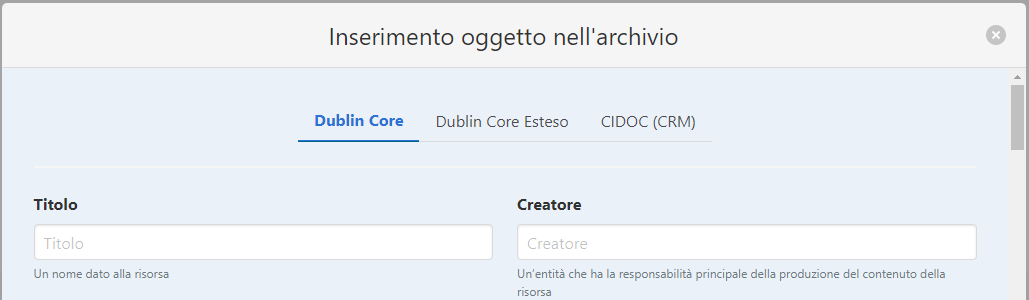
\includegraphics[width=1\textwidth]{immagini/inserimentoArchivio.PNG}
\caption{Progetto: Modulo inserimento nell'archivio}
\label{fig:progettoInserimento}
\end{figure}

La prima opzione, "Dublin Core", fornisce quindici etichette base per la descrizione delle risorse. La seconda opzione, "Dublin Core Esteso", permette una descrizione più approfondita della risorsa attraverso l'uso di qualificatori (o sottoclassi) che permettono un raffinamento dello schema con l'aggiunta di significati più precisi sui termini base. Infine la terza opzione, "CIDOC", è rivolta agli "esperti" in quanto fornisce un modello ontologico formale incentrato sulla rappresentazione semantica delle risorse.

Un ultima considerazione pratica riguarda le linee guida per la descrizione di beni culturali, fornite dal nucleo carabinieri per la tutela del patrimonio culturale in figura \ref{fig:carabinieriTPC}.

\begin{figure}[H]
\centering
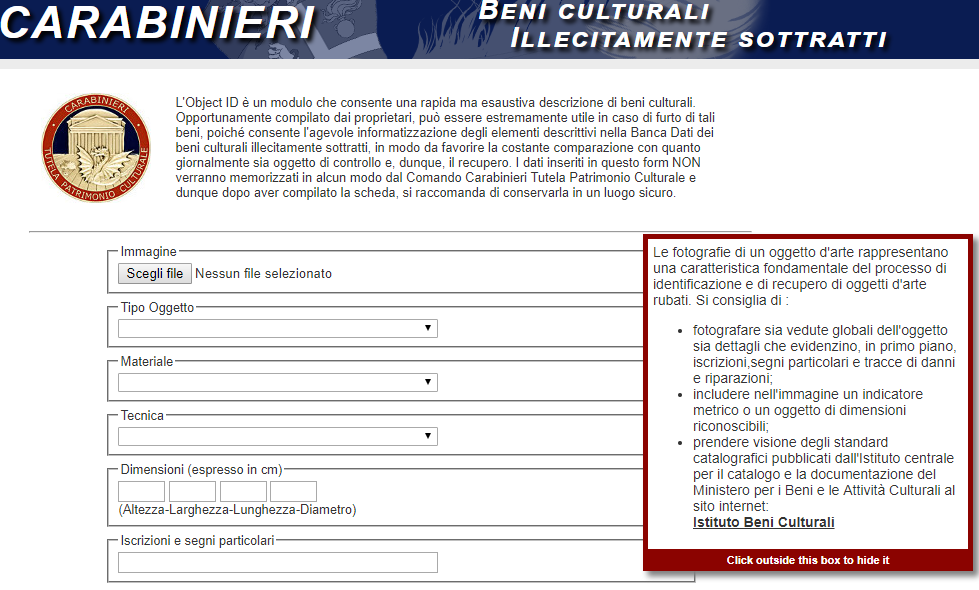
\includegraphics[width=1\textwidth]{immagini/carabinieriTPC2.png}
\caption{Beni culturali illecitamente sottratti: Modulo descrittivo}
\label{fig:carabinieriTPC}
\end{figure}

Il modulo Object ID\footfullcite{tpcCarabinieri} consente la descrizione di beni culturali ed è utile per le operazioni di recupero in caso di furto di tali beni. Idealmente quando la tecnologia sarà sufficientemente matura e testata, l'approvazione degli oggetti inseriti tramite un'applicazione basata sulla blockchain, potrebbe essere fatta dai membri autorizzati del Comando Carabinieri. Chiaramente il fatto di poter contare su una base di dati immutabile, permanente e dotata di storia completa fornirebbe dei vantaggi rilevanti rispetto ai sistemi attualmente in uso.

Dunque con questo progetto si vuole dimostrare che è possibile adottare qualunque schema di descrizione in maniera relativamente semplice e quindi fornire una prova attendibile del possesso di tali beni. Mentre queste considerazioni sono state fatte tenendo in mente l'obiettivo consistente nella dimostrazione della metodologia, nel caso di un’applicazione pronta ad essere adottata al pubblico, questa parte assumerebbe un ruolo di primo piano per l'intero processo di sviluppo.

\section{Preparazione dell'ambiente di sviluppo}

Lo sviluppo del progetto sulla blockchain Ethereum è accompagnato dalla presenza di numerosi strumenti forniti dalla comunità, in questa sezione sarà fornita la lista dei principali strumenti e delle dipendenze utilizzate durante la programmazione.

\begin{itemize}
\item NPM (Node Package Manager) per la gestione e l'installazione dei moduli/librerie Javascript. NPM richiede la presenza di Node.js\footnote{In questo progetto si è utilizzato Node.js nella versione 10.8.0 e NPM versione 6.2.0}.
\item Truffle framework (versione 4.1.14)\footfullcite{truffleFramework} un ambiente di sviluppo composto da un insieme di strumenti che facilitano la creazione delle applicazioni decentralizzate (di seguito dApps) sulla piattaforma Ethereum. Truffle gestisce il ciclo di migrazione (sulla blockchain) degli smart contracts, il funzionamento dei contratti e l'esecuzione di test automatizzati.

Il framework include Ganache\footfullcite{ganache} (versione 1.2.2), una blockchain personale, utile per lo sviluppo locale delle dApps. Ganache è un emulatore di nodi Ethereum con un'interfaccia grafica (in figura {\ref{fig:ganache}}) intuitiva, mette a disposizione un certo numero di account precaricati con Ether. Si tratta di una blockchain con un funzionamento semplificato permette di analizzare lo stato della blockchain.

\begin{figure}[H]
\centering
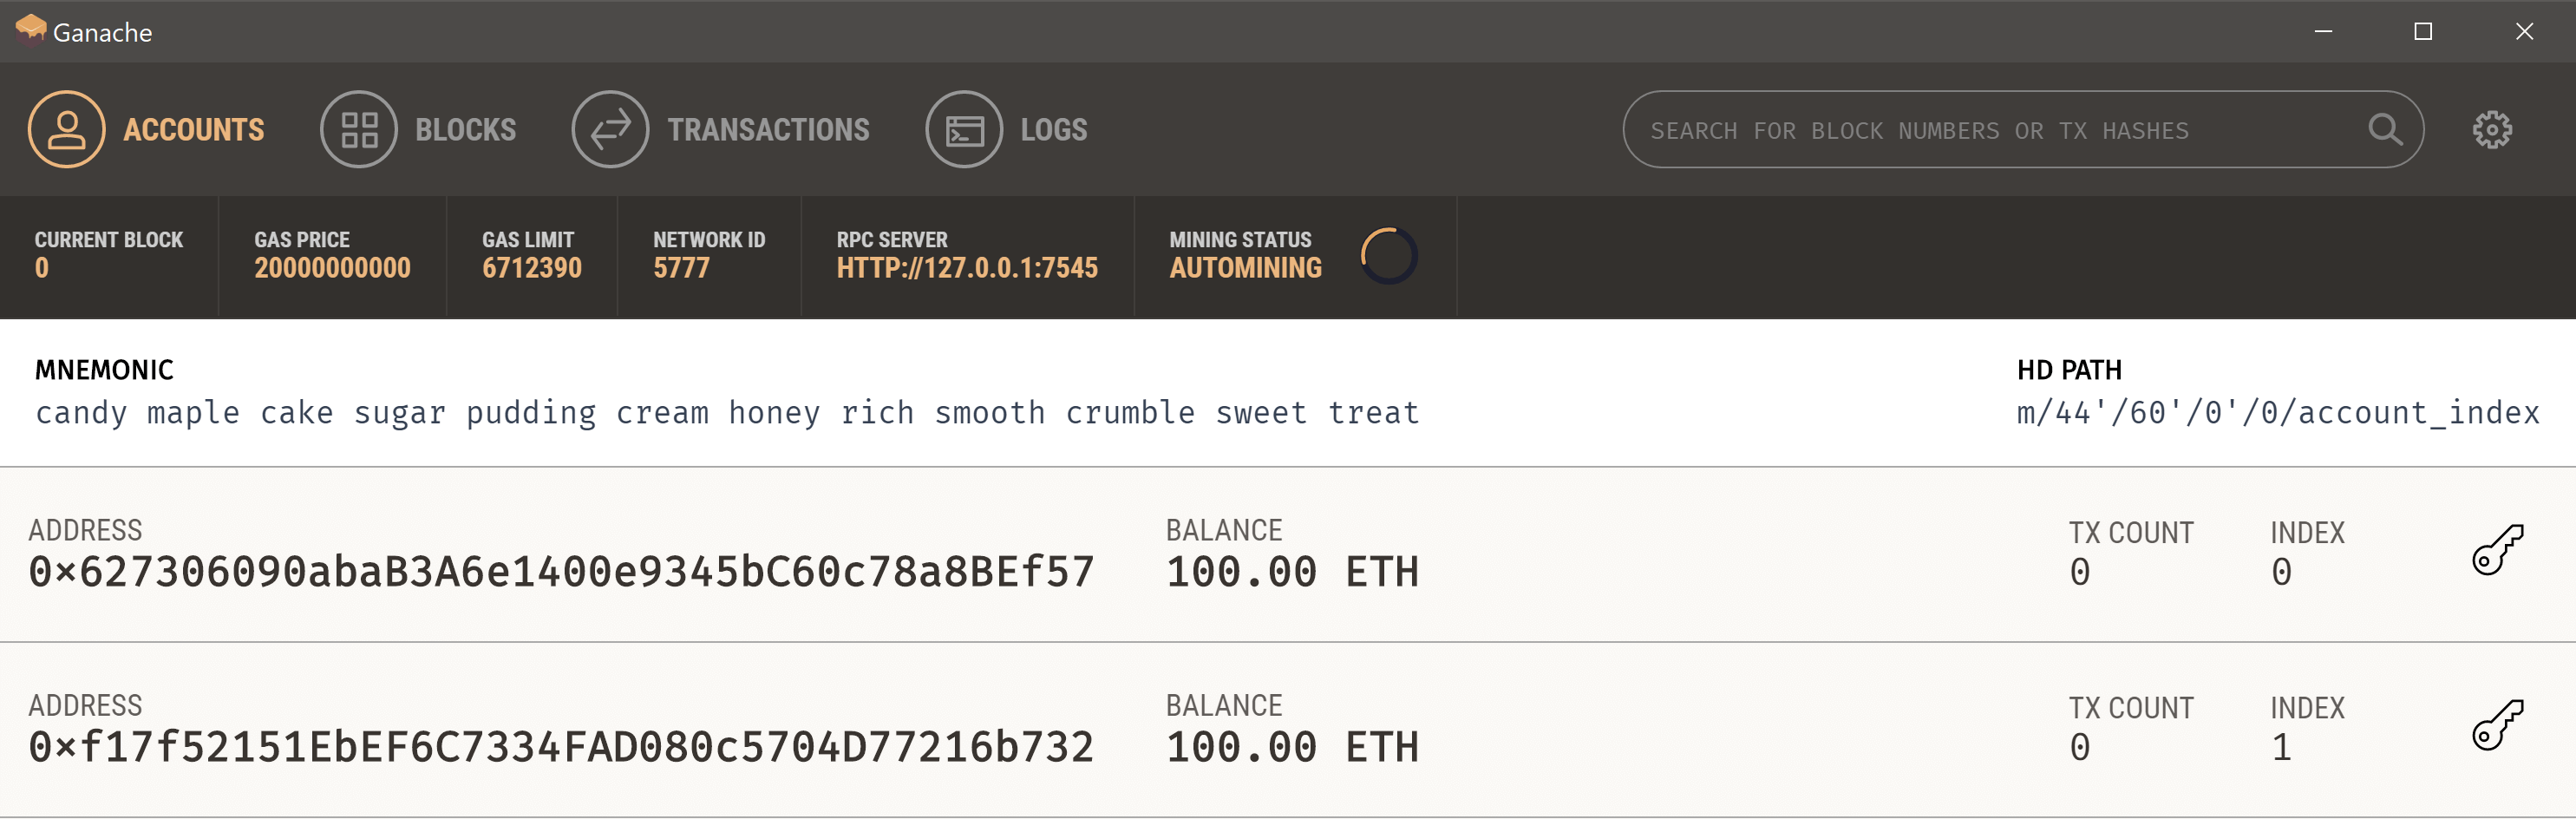
\includegraphics[width=1\textwidth]{immagini/ganache-window.png}
\caption{Ganache: Blockchain locale}
\label{fig:ganache}
\end{figure}

Truffle fornisce anche \emph{boilerplates} chiamati "boxes" utili per uno sviluppo accelerato\footnote{Come base di questo progetto si è scelto il pacchetto chiamato pet-shop disponibile su https://truffleframework.com/boxes/pet-shop}. 
\item Mocha e Chai
\item Metamask
\item Web3.js
\end{itemize}




\section{Sviluppo dell'applicazione}
MVP..
\subsection{Scrittura dei Contratti}

\subsection{Fase di test}

\subsection{Testnet}

\subsection{Programmazione front-end}

\subsection{Ethereum Testnet}

\subsection{Considerazioni finali}


